\documentclass{article}
    \usepackage[utf8]{inputenc}
    \usepackage{tikz}
    \usepackage{xcolor}
    \usepackage{graphicx}
    \usepackage{amsmath}
    \usepackage{caption}

    \definecolor{brightmaroon}{RGB}{195,33,72}
    \definecolor{cyan}{RGB}{0,255,255}
    \definecolor{skyblue}{RGB}{135,206,235}

    \begin{document}
    \begin{figure}[htbp]
        \centering
        \resizebox{.75\linewidth}{!}{
            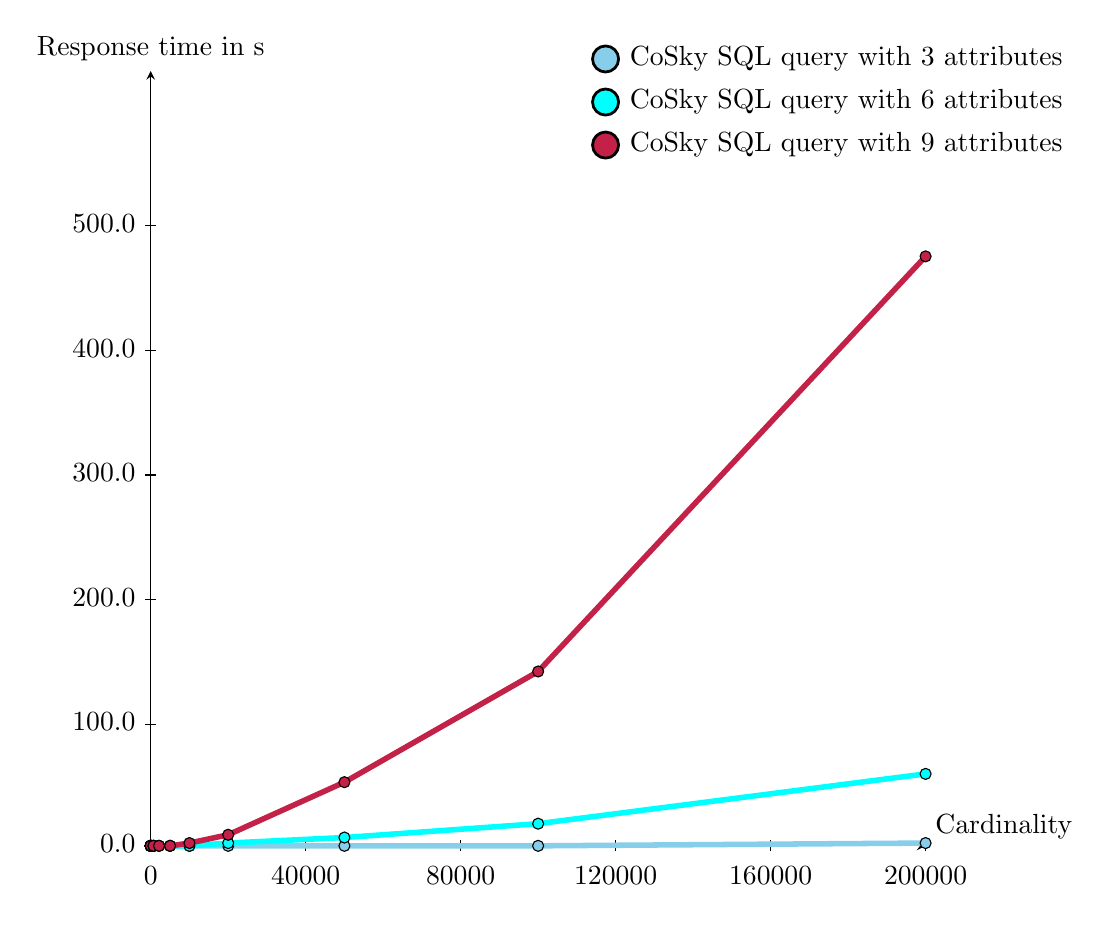
\begin{tikzpicture}[line join=bevel,
                bigbrightmaroonnode/.style={shape=circle, fill=brightmaroon, draw=black, line width=1pt},
                bigcyannode/.style={shape=circle, fill=cyan, draw=black, line width=1pt},
                bigskybluenode/.style={shape=circle, fill=skyblue, draw=black, line width=1pt}]
            % Axes
            \draw[-stealth] (0pt, 0pt) -- (280pt, 0pt) node[anchor=north west, yshift=15pt] {Cardinality};
            \draw[-stealth] (0pt, 0pt) -- (0pt, 280pt) node[anchor=south] {Response time in s};
            % X-axis ticks
        \foreach \x/\xtext in {
            0pt/$0$,
            56pt/$40000$,
            112pt/$80000$,
            168pt/$120000$,
            224pt/$160000$,
            280pt/$200000$} {
            \draw (\x, 2pt) -- (\x, -2pt) node[below] {\xtext\strut};
        }
        % Y-axis ticks
        \foreach \y/\ytext in {
            0pt/$0.0$,
            44pt/$100.0$,
            89pt/$200.0$,
            134pt/$300.0$,
            179pt/$400.0$,
            224pt/$500.0$} {
            \draw (2pt, \y) -- (-2pt, \y) node[left] {\ytext\strut};
        }
        \draw[skyblue, line width=2pt] (0pt, 0pt) -- (0pt, 0pt) -- (0pt, 0pt) -- (0pt, 0pt) -- (0pt, 0pt) -- (1pt, 0pt) -- (1pt, 0pt) -- (3pt, 0pt) -- (7pt, 0pt) -- (14pt, 0pt) -- (28pt, 0pt) -- (70pt, 0pt) -- (140pt, 0pt) -- (280pt, 1pt);
        \filldraw[color=black, fill=skyblue] (0pt, 0pt) circle (2pt);
        \filldraw[color=black, fill=skyblue] (0pt, 0pt) circle (2pt);
        \filldraw[color=black, fill=skyblue] (0pt, 0pt) circle (2pt);
        \filldraw[color=black, fill=skyblue] (0pt, 0pt) circle (2pt);
        \filldraw[color=black, fill=skyblue] (0pt, 0pt) circle (2pt);
        \filldraw[color=black, fill=skyblue] (1pt, 0pt) circle (2pt);
        \filldraw[color=black, fill=skyblue] (1pt, 0pt) circle (2pt);
        \filldraw[color=black, fill=skyblue] (3pt, 0pt) circle (2pt);
        \filldraw[color=black, fill=skyblue] (7pt, 0pt) circle (2pt);
        \filldraw[color=black, fill=skyblue] (14pt, 0pt) circle (2pt);
        \filldraw[color=black, fill=skyblue] (28pt, 0pt) circle (2pt);
        \filldraw[color=black, fill=skyblue] (70pt, 0pt) circle (2pt);
        \filldraw[color=black, fill=skyblue] (140pt, 0pt) circle (2pt);
        \filldraw[color=black, fill=skyblue] (280pt, 1pt) circle (2pt);

        \draw[cyan, line width=2pt] (0pt, 0pt) -- (0pt, 0pt) -- (0pt, 0pt) -- (0pt, 0pt) -- (0pt, 0pt) -- (1pt, 0pt) -- (1pt, 0pt) -- (3pt, 0pt) -- (7pt, 0pt) -- (14pt, 0pt) -- (28pt, 1pt) -- (70pt, 3pt) -- (140pt, 8pt) -- (280pt, 26pt);
        \filldraw[color=black, fill=cyan] (0pt, 0pt) circle (2pt);
        \filldraw[color=black, fill=cyan] (0pt, 0pt) circle (2pt);
        \filldraw[color=black, fill=cyan] (0pt, 0pt) circle (2pt);
        \filldraw[color=black, fill=cyan] (0pt, 0pt) circle (2pt);
        \filldraw[color=black, fill=cyan] (0pt, 0pt) circle (2pt);
        \filldraw[color=black, fill=cyan] (1pt, 0pt) circle (2pt);
        \filldraw[color=black, fill=cyan] (1pt, 0pt) circle (2pt);
        \filldraw[color=black, fill=cyan] (3pt, 0pt) circle (2pt);
        \filldraw[color=black, fill=cyan] (7pt, 0pt) circle (2pt);
        \filldraw[color=black, fill=cyan] (14pt, 0pt) circle (2pt);
        \filldraw[color=black, fill=cyan] (28pt, 1pt) circle (2pt);
        \filldraw[color=black, fill=cyan] (70pt, 3pt) circle (2pt);
        \filldraw[color=black, fill=cyan] (140pt, 8pt) circle (2pt);
        \filldraw[color=black, fill=cyan] (280pt, 26pt) circle (2pt);

        \draw[brightmaroon, line width=2pt] (0pt, 0pt) -- (0pt, 0pt) -- (0pt, 0pt) -- (0pt, 0pt) -- (0pt, 0pt) -- (1pt, 0pt) -- (1pt, 0pt) -- (3pt, 0pt) -- (7pt, 0pt) -- (14pt, 1pt) -- (28pt, 4pt) -- (70pt, 23pt) -- (140pt, 63pt) -- (280pt, 213pt);
        \filldraw[color=black, fill=brightmaroon] (0pt, 0pt) circle (2pt);
        \filldraw[color=black, fill=brightmaroon] (0pt, 0pt) circle (2pt);
        \filldraw[color=black, fill=brightmaroon] (0pt, 0pt) circle (2pt);
        \filldraw[color=black, fill=brightmaroon] (0pt, 0pt) circle (2pt);
        \filldraw[color=black, fill=brightmaroon] (0pt, 0pt) circle (2pt);
        \filldraw[color=black, fill=brightmaroon] (1pt, 0pt) circle (2pt);
        \filldraw[color=black, fill=brightmaroon] (1pt, 0pt) circle (2pt);
        \filldraw[color=black, fill=brightmaroon] (3pt, 0pt) circle (2pt);
        \filldraw[color=black, fill=brightmaroon] (7pt, 0pt) circle (2pt);
        \filldraw[color=black, fill=brightmaroon] (14pt, 1pt) circle (2pt);
        \filldraw[color=black, fill=brightmaroon] (28pt, 4pt) circle (2pt);
        \filldraw[color=black, fill=brightmaroon] (70pt, 23pt) circle (2pt);
        \filldraw[color=black, fill=brightmaroon] (140pt, 63pt) circle (2pt);
        \filldraw[color=black, fill=brightmaroon] (280pt, 213pt) circle (2pt);

        % Caption
            \matrix [below left] at (current bounding box.north east) {
                \node [bigskybluenode, label=right:CoSky SQL query with 3 attributes] {}; \\
            \node [bigcyannode, label=right:CoSky SQL query with 6 attributes] {}; \\
            \node [bigbrightmaroonnode, label=right:CoSky SQL query with 9 attributes] {}; \\
        };
            \end{tikzpicture}
        }
        \caption{Execution time of CoSky SQL queries with 3, 6, and 9 attributes}
        \label{fig:cosky_sql_comparaison}
    \end{figure}
    \end{document}